\documentclass[main.tex]{subfiles}
% 线性变换的定义和基本性质
\begin{document}
在本节我们考虑由一个向量空间到另一个向量空间的一种映射。我们先限定,建立了映射的两个向量空间是在同一数域上的。

向量空间是含有运算规则规定的集合。由一个向量空间到另一个向量空间的映射不一定能保持运算规则不变。所谓保持运算规则不变,意思就是定义域所在空间的运算法则,经过映射之后的陪域也具备。比如说,如果$f\left(\alpha\mathbf{a}+\beta\mathbf{b}\right)=\alpha f\left(\mathbf{a}\right)+\beta f\left(\mathbf{b}\right)$,则在一个向量空间上的映射$f$的陪域也是一个向量空间。这当然不是一定能保证的。如果两个同类代数结构之间的映射保持这类代数结构的关系定义不变,则称这种映射为这类代数结构上的\emph{同态映射(homomorphism)}。
\begin{example}
    以下映射是否向量空间上的同态映射?
    \begin{itemize}
        \item $f:\mathbb{R}\rightarrow\mathbb{R}:f\left(x\right)=x^2$
              讨论过程:$x\in\mathbb{R}$,视$\mathbb{R}$为数域$\mathbb{R}$上的向量空间,想要映射$f$是同态的,需要其满足$f\left(\alpha x+ y\right)=\alpha f\left(x\right)+f\left(y\right),\quad\forall x,y,\alpha\in\mathbb{R}$。显然,本例中的映射$f$并不满足。
        \item $g:\mathbb{R}^2\rightarrow\mathbb{R}:g\left(x,y\right)=x^2+y^2-4$
        \item $F:\mathbb{R}^2\rightarrow\mathbb{C}:F\left(x,y\right)=U\left(x,y\right)+iV\left(x,y\right),U,V:\mathbb{R}^2\rightarrow\mathbb{R}$
        \item $T:\mathbb{R}\rightarrow\mathbb{R}^2:T\left(t\right)=\left(t+3,2t-5\right)$
        \item 一个点粒子在空间中的运动可视为一个映射$M:\left[a,b\right]\rightarrow\mathbb{R}^3$,具体定义为对每一$t\in\left[a,b\right],M\left(t\right)=\left(x\left(t\right),y\left(t\right),z\left(t\right)\right)$,其中$x\left(t\right),y\left(t\right),z\left(t\right)$是$t$的实值函数。如果视$t$为时间,则$M\left(t\right)$描述了粒子的运动轨迹,$a$和$b$是运动的起始和终止时间。
    \end{itemize}
\end{example}

\begin{definition}[线性变换]\label{def:II.2.11}
    设$\mathcal{V}$和$\mathcal{W}$是$\mathbb{F}$上的向量空间。如果从$\mathcal{V}$到$\mathcal{W}$的映射$T:\mathcal{V}\rightarrow\mathcal{W}$满足
    \[T\left(\alpha\mathbf{a}+\beta\mathbf{b}\right)=\alpha T\left(\mathbf{a}\right)+\beta T\left(\mathbf{b}\right)\]
    则称$T$是从$\mathcal{V}$到$\mathcal{W}$的线性变换(linear transformation),常写成算符的形式:$T\left(\mathbf{a}\right)=\mathbf{Ta}$。如果两个线性变换$\mathbf{T}:\mathcal{V}\rightarrow\mathcal{W}$和$\mathbf{U}:\mathcal{V}\rightarrow\mathcal{W}$满足$\mathbf{Ta}=\mathbf{Ua}\forall\mathbf{a}\in\mathcal{V}$则称这两个线性变换相等,$\mathbf{U}=\mathbf{T}$。零变换$\mathbf{T}_0:\mathcal{V}\rightarrow\mathcal{W}$定义为$\mathbf{T}_0\mathbf{a}=\mathbf{0}_\mathcal{W}\forall\mathbf{a}\in\mathcal{V}$,其中$\mathbf{0}_\mathcal{W}\in\mathcal{W}$表示$\mathcal{W}$中的零向量\footnote{此处要注意区分不同向量空间中的零向量。}。
\end{definition}

注意,定义\ref{def:II.2.11}除了说线性变换是向量空间上的同态映射之外,还有其他的规定。由定义\ref{def:II.2.11},可直接证得以下结论:
\begin{itemize}
    \item 任何一个线性变换都总把零向量映射为零向量。
    \item 两个向量空间之间的恒等映射是$\mathcal{V}$到其自身的线性变换$\mathbf{I}_\mathcal{V}:\mathcal{V}\rightarrow\mathcal{V},\mathbf{I}_\mathcal{V}\mathbf{a}=\mathbf{a}\forall\mathbf{a}\in\mathcal{V}$又可称为恒等线性变换。
\end{itemize}

正如由定义\ref{def:II.2.1}所定义的向量那般,定义\ref{def:II.2.11}定义的线性变换也是抽象概念。在例\ref{exp:II.2.1}中的向量空间上都可以建立线性变换。

\begin{example}\label{exp:II.2.9}
    \begin{itemize}
        \item 回顾课本《线性代数与解析几何》相关例题\cite{周胜林2012线性代数}[\S 7.1例题1.4、\S 7.3例题3.3]。这些例题说明求导运算是线性的。
        \item 设$\mathcal{V}$是所有由$\mathbb{R}$到$\mathbb{R}$的连续函数的集合,验证$\mathcal{V}$是实数域$\mathbb{R}$上的向量空间。定义$\mathcal{V}$上的映射$T$,对任意$\mathcal{V}$中的向量$f$,$\left(Tf\right)\left(x\right)\equiv\int_0^x f\left(t\right)\mathrm{d}t,\forall x\in\mathbb{R},f\in\mathcal{V}$,验证$T$是由$\mathcal{V}$到$\mathcal{V}$的线性变换。这一例子说明积分运算是线性的。
    \end{itemize}
\end{example}

% 留作业:H&K p.73#1

下面这个定理,使得线性变换本身也能形成一个向量空间(见推论)。

\begin{theorem}\label{thm:II.2.6}
    设$\mathcal{V}$、$\mathcal{W}$是$\mathbb{F}$上的向量空间,$\mathbf{T}$、$\mathbf{U}$是从$\mathcal{V}$到$\mathcal{W}$的线性变换。若定义
    \[\left(\mathbf{T}+\mathbf{U}\right)\mathbf{a}=\mathbf{Ta}+\mathbf{Ua},\forall\mathbf{a}\in\mathcal{V}\]
    \[\left(\alpha\mathbf{T}\right)\mathbf{a}=\alpha\left(\mathbf{Ta}\right),\forall\alpha\in\mathbb{F}\]
    则$\left(\mathbf{T}+\mathbf{U}\right)$和$\alpha\mathbf{T}$也是从$\mathcal{V}$到$\mathcal{W}$的线性变换。
\end{theorem}
\begin{proof}
    分别用$\mathbf{T}+\mathbf{U}$和$\alpha\mathbf{T}$作用于向量$\beta\mathbf{a}+\gamma\mathbf{b},\alpha,\beta\in\mathbb{F},\mathbf{a},\mathbf{b}\in\mathcal{V}$,使用向量空间的定义\ref{def:II.2.1}、线性变换的定义\ref{def:II.2.11}和本命题中的运算定义证明。略。
\end{proof}

\begin{corollary}
    给定数域$\mathbb{F}$上的两个向量空间$\mathcal{V},\mathcal{W}$,所有由$\mathcal{V}$到$\mathcal{W}$的线性变换的集合是一个数域$\mathbb{F}$上的向量空间,记为$\mathcal{L}\left(\mathcal{V},\mathcal{W}\right)$,零变换是该向量空间的零向量。
\end{corollary}
\begin{proof}
    前一句由定理\ref{thm:II.2.6}易证。设$\mathbf{T}_0$是由$\mathcal{V}$到$\mathcal{W}$的零变换,对任一$\mathbf{T}\in\mathcal{L}\left(\mathcal{V},\mathcal{W}\right)$和$\mathbf{a}\in\mathcal{V}$,$\left(\mathbf{T}_0+\mathbf{T}\right)\mathbf{a}=\mathbf{T}_0\mathbf{a}+\mathbf{Ta}=\mathbf{0}_\mathcal{W}+\mathbf{Ta}=\mathbf{Ta}$,即$\mathbf{T}_0+\mathbf{T}=\mathbf{T}\forall\mathbf{T}\in\mathcal{L}\left(\mathcal{V},\mathcal{W}\right)$。
\end{proof}

请读者按照向量空间的定义验证,线性变换的空间$\mathcal{L}\left(\mathcal{V},\mathcal{W}\right)$作为一个向量空间,拥有一切向量空间的一般性质。注意:在记法$\mathcal{L}\left(\mathcal{V},\mathcal{W}\right)$中,括号表示有序对。

接下来,我们先考察$\mathcal{L}\left(\mathcal{V},\mathcal{W}\right)$的基和维数。不关心证明的读者可直接朗读定理\ref{thm:II.2.7}。

\begin{lemma}\label{lem:II.2.1}
    设$\mathcal{V}_N$是数域$\mathbb{F}$上的$N$维向量空间,$B_\mathcal{V}=\left\{\mathbf{e}_i\right\}_{i=1}^N$是$\mathcal{V}_N$的一组基,$\mathcal{W}$是同数域上的另一向量空间。对$\mathcal{W}$中给定的任意一组$N$个不同向量$\left\{\mathbf{b}_i\right\}_{i=1}^N\in\mathcal{W}$,有且只有一个线性变换$\mathbf{T}:\mathcal{V}_N\rightarrow\mathcal{W}$满足$\mathbf{Te}_i=\mathbf{b}_i,i=1,\cdots,N$。
\end{lemma}
\begin{proof}
    存在性的证明,只需找出这一线性变换。任一$\mathbf{a}\in\mathcal{V}_N$可用基$B_\mathcal{V}$表示成
    \[\mathbf{a}=\sum_{i=1}^N\alpha_i\mathbf{e}_i,\alpha_i\in\mathbb{F},i=1,\cdots,N\]
    特别地,
    \[\mathbf{e}_i=\sum_{j=1}^N\delta_{ij}\mathbf{e}_j,i=1,\cdots,N\]
    定义映射$\mathbf{T}:\mathcal{V}_N\rightarrow\mathcal{W},\mathbf{Ta}\equiv\sum_{i=1}^N\alpha_i\mathbf{b}_i$,则易验$\mathbf{Te}_i=\mathbf{b}_i,i=1,\cdots,N$。我们还需验证映射$\mathbf{T}$是线性变换,按定义\ref{def:II.2.11}只需验证$T\left(\alpha\mathbf{a}+\beta\mathbf{b}\right)=\alpha\left(\mathbf{Ta}\right)+\beta\left(\mathbf{Tb}\right)$即可。给定任意$\mathbf{b}\in\mathcal{V}_N$和标量$\gamma\in\mathbb{F}$,其中$\mathbf{b}$可表示为$\mathbf{b}=\sum_{i=1}^N\beta_i\mathbf{e}_i$,且有
    \[\gamma\mathbf{a}+\mathbf{b}=\sum_{i=1}^N\left(\gamma\alpha_i+\beta_i\right)\mathbf{e}_i\]
    由$\mathbf{T}$的定义有
    \begin{align}
        \mathbf{T}\left(\gamma\mathbf{a}+\mathbf{b}\right) & =\sum_{i=1}^N\left(\gamma\alpha_i+\beta_i\right)\mathbf{b}_i            \\
        \gamma\left(\mathbf{Ta}\right)+\mathbf{Tb}         & =\gamma\sum_{i=1}^N\alpha_i\mathbf{b}_i+\sum_{i=1}^N\beta_i\mathbf{b}_i \\
                                                           & =\sum_{i=1}^N\left(\gamma\alpha_i+\beta_i\right)\mathbf{b}_i
    \end{align}
    所以$\mathbf{T}\left(\gamma\mathbf{a}+\mathbf{b}\right)=\gamma\left(\mathbf{Ta}\right)+\mathbf{Tb}$对任意向量$\mathbf{a},\mathbf{b}\in\mathcal{V}_N$和标题$\gamma\in\mathbb{F}$均成立,即$\mathbf{T}$是一个线性变换。存在性证毕。

    唯一性的证明,设另有一线性变换$\mathbf{U}:\mathcal{V}_N\rightarrow\mathcal{W}$也满足$\mathbf{Ue}_i=\mathbf{b}_i$,则对任一$\mathbf{a}\in\mathcal{V}_N$,
    \[
        \mathbf{Ua}=\mathbf{U}\left(\sum_{i=1}^N\alpha_i\mathbf{e}_i\right)=\sum_{i=1}^N\alpha_i\mathbf{Ue}_i=\sum_{i=1}^N\alpha_i\mathbf{b}_i\]
    即$\mathbf{U}$就是$\mathbf{T}$。
\end{proof}

\begin{theorem}\label{thm:II.2.7}
    若$\mathcal{V}_N,\mathcal{W}_M$分别为数域$\mathbb{F}$上的$N,M$维向量空间,则$\mathcal{L}\left(\mathcal{V}_N,\mathcal{W}_M\right)$的维数是$M\times N$。
\end{theorem}
\begin{proof}
    证明的过程,相当于找出$\mathcal{L}\left(\mathcal{V}_N,\mathcal{W}_M\right)$的基\footnote{我们在例\ref{exp:II.2.6}中找过数域$\mathbb{F}$上的$n\times n$矩阵空间的一组规范正交基$\left\{E^{pq}\right\}_{p,q=1}^n$。定理\ref{thm:II.2.7}的证明过程与例\ref{exp:II.2.6}很类似。}

    设$B_\mathcal{V}=\left\{\mathbf{e}_i\right\}_{i=1}^N,B_\mathcal{W}=\left\{\mathbf{f}_j\right\}_{j=1}^M$分别为$\mathcal{V}_N,\mathcal{W}_M$的基。对于每一对整数$\left(p,q\right),1\leq p\leq N,1\leq q\leq M$,定义一个线性变换$\mathbf{E}^{pq}:\mathcal{V}_N\rightarrow\mathcal{W}_M$
    \[
        \mathbf{E}^{pq}\mathbf{e}_i=\left\{\begin{array}{cc}
            \mathbf{0}_\mathcal{W}, & i\neq p \\
            \mathbf{f}_q,           & i=p
        \end{array}\right.
    \]
    给定任一线性变换$\mathbf{T}\in\mathcal{L}\left(\mathcal{V}_N,\mathcal{W}_M\right)$,且令
    \[\mathbf{Te}_i=\sum_{q=1}^MA_{qi}\mathbf{f}_q\]
    由引理\ref{lem:II.2.1},对$\left\{\mathbf{f}_j\right\}_{j=1}^M$,满足上式的$\mathbf{T}$是唯一的,且根据向量的坐标表达式,上式中的$A_{qi}$就是向量$\mathbf{Te}_i$在有序基$B_\mathcal{W}$下的坐标。

    下面我们证明$\mathbf{T}$能被$\left\{\mathbf{E}^{pq}\right\}$线性表出。定义$\mathbf{U}\in\mathcal{L}\left(\mathcal{V}_N,\mathcal{W}_M\right)$,$\mathbf{Ue}_i=\sum_p\sum_qA_{qp}\mathbf{E}^{pq}\mathbf{e}_i$,则
    \begin{align*}
        \mathbf{Ue}_i & =\sum_p\sum_qA_{qp}\mathbf{E}^{pq}\mathbf{e}_i \\
                      & =\sum_p\sum_qA_{qp}\delta_{ip}\mathbf{f}_q     \\
                      & =\sum_qA_{qi}\mathbf{f}_q                      \\
                      & =\mathbf{Te}_i
    \end{align*}
    则可见$\mathbf{U}=\mathbf{T}$,同时有
    \[\mathbf{T}=\sum_{p=1}^N\sum_{q=1}^MA_{qp}\mathbf{E}^{pq}\]
    由于$\mathbf{T}$是$\mathcal{L}\left(\mathcal{V}_N,\mathcal{W}_M\right)$中的任意一个线性变换,故$\mathcal{L}\left(\mathcal{V}_N,\mathcal{W}_M\right)$是$\left\{\mathbf{E}^{pq}\right\}$的线性生成空间。由基的定义\ref{def:II.2.5},现在我们只需再证$\left\{\mathbf{E}^{pq}\right\}$是线性无关的,它们就是$\mathcal{L}\left(\mathcal{V}_N,\mathcal{W}_M\right)$的基了。按照线性无关的定义,设$\mathbf{T}$是零变换,由于$\left\{\mathbf{f}_j\right\}_{j=1}^M$是线性无关的,故有
    \[\mathbf{T}=\mathbf{0}=\sum_{p=1}^N\sum_{q=1}^MA_{qp}\mathbf{E}^{pq}\Leftrightarrow\mathbf{Te}_i=\sum_q A_{qi}\mathbf{f}_q=\mathbf{0}_\mathcal{W}\Leftrightarrow A_{qi}=0\forall q=1,\cdots,M,i=1,\cdots,N\]
    即$\left\{\mathbf{E}^{pq}\right\}$线性无关。故$\left\{\mathbf{E}^{pq}\right\}$是$\mathcal{L}\left(\mathcal{V}_N,\mathcal{W}_M\right)$的一组基,$\mathcal{L}\left(\mathcal{V}_N,\mathcal{W}_M\right)$的维数就是$M\times N$。
\end{proof}

注意,给定两个有限维向量空间$\mathcal{V},\mathcal{W}$,$\mathcal{L}\left(\mathcal{V},\mathcal{W}\right)$中的线性变换和$\mathcal{L}\left(\mathcal{W},\mathcal{V}\right)$中的线性变换是不同空间的元素,没有一般关系——虽然它们的维数无非只是$M\times N$和$N\times M$的差别。

讨论完线性变换本身作为向量的性质——它所在向量空间的基与维数,我们接下来转而考虑线性变换作为映射的性质:单射、满射、双射……。线性变换作为映射的性质与它所映射的两个向量空间的维数有关,这是线性代数最重要的定理之一——线性变换的维数定理。下面我们先为该定理的引入介绍一些必要概念。

\begin{definition}[零空间、零化度、秩]\label{def:II.2.12}
    (如图\ref{fig:II.2.1}所示)设$\mathcal{V}$和$\mathcal{W}$是数域$\mathbb{F}$上的向量空间。线性变换$\mathbf{T}:\mathcal{V}\rightarrow\mathcal{W}$的\emph{零空间(null space)}或\emph{核空间(kernel)}是所有满足$\mathbf{Ta}=\mathbf{0}_\mathcal{W}$的向量$\mathbf{a}$的集合,记作$\mathrm{ker}\mathbf{T}$。零空间的维数称为该线性变换的\emph{零化度(nullity)},记作$\mathrm{nullity}\mathbf{T}\equiv\mathrm{dim}\left(\mathrm{ker}\mathbf{T}\right)$。如果$\mathcal{V}$是有限维向量空间,则$\mathbf{T}$的\emph{秩(rank)}是$\mathbf{T}$的值域的维数,记作$\mathrm{rank}\mathbf{T}\equiv\mathrm{dim}\left(\mathrm{ran}\mathbf{T}\right)$。特别地,如果$\mathrm{nullity}\mathbf{T}=0$,即$\mathbf{T}$的零空间只有零向量$\mathbf{0}_\mathcal{V}$一个元素,则称$\mathbf{T}$是\emph{非奇异的(non-singular)}。
\end{definition}

\begin{figure}[htbp]
    \centering
    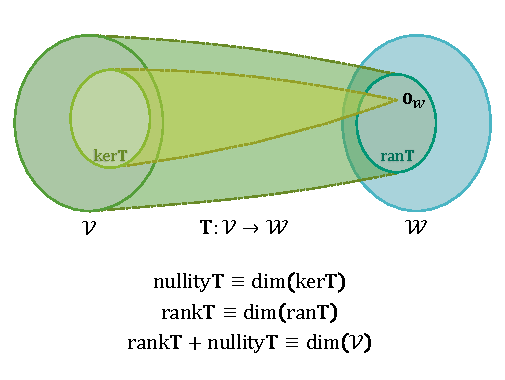
\includegraphics{images/II.2.1.pdf}
    \caption{线性变换的零空间、值域、零化度和秩以及线性变换的维数定理}
    \label{fig:II.2.1}
\end{figure}

上述定义默认了两个易验事实的成立:$\mathrm{ker}\mathbf{T}$是$\mathcal{V}$的子空间,$\mathrm{ran}\mathbf{T}$是$\mathcal{W}$的子空间(否则不能直接谈它这两个子集的“维数”),证明从略\cite[\S7.3“2.线性变换的简单性质(4)”]{周胜林2012线性代数}。

基于定义\ref{def:II.2.12}的概念,我们给出线性代数中非常重要的定理——线性变换的维数定理\footnote{\cite[\S7.3 “2.线性变换的简单性质(5)”]{周胜林2012线性代数}}。

\begin{theorem}[线性变换的维数定理]\label{thm:II.2.8}
    设$\mathcal{V}$和$\mathcal{W}$是数域$\mathbb{F}$上的向量空间,其中$\mathcal{V}$是有限维向量空间,则对线性变换$\mathbf{T}:\mathcal{V}\rightarrow\mathcal{W}$有
    \[
        \mathrm{rank}\mathbf{T}+\mathrm{nullity}\mathbf{T}=\mathrm{dim}\mathcal{V}
    \]
\end{theorem}
\begin{proof}
    设$\mathrm{dim}\mathcal{V}=n$,$\mathrm{nullity}\mathbf{T}=\mathrm{dim}\left(\mathrm{ker}\mathbf{T}\right)=k$,$\left\{\mathbf{a}_1,\cdots,\mathbf{a}_k\right\}$是$\mathrm{ker}\mathbf{T}$的一组基。则可在$\mathcal{V}$中继续找到$\left\{\mathbf{a}_{k+1},\cdots,\mathbf{a}_{n}\right\}$与$\left\{\mathbf{a}_1,\cdots,\mathbf{a}_k\right\}$合并成线性无关向量组,从而成为$\mathcal{V}$的基。

    由于$\left\{\mathbf{Ta}_1,\cdots,\mathbf{Ta}_n\right\}$线性生成$\mathbf{T}$的值域$\mathrm{ran}\mathbf{T}$(由线性变换性质易证),其中由于$\left\{\mathbf{a}_1,\cdots,\mathbf{a}_k\right\}\in\mathrm{ker}\mathbf{T}$,故有$\mathbf{Ta}_j=\mathbf{0}_\mathcal{W}\forall j\leq k$,所以实际上仅$\left\{\mathbf{Ta}_{k+1},\cdots,\mathbf{Ta}_n\right\}$就线性生成$\mathrm{ran}\mathbf{T}$了。我们进一步验证它们是线性无关的。设标量$\gamma_i$满足$\sum_{i=k+1}^n\gamma_i\mathbf{Ta}_i=\mathbf{0}_\mathcal{W}$,即
    \[\mathbf{T}\left(\sum_{i=k+1}^n\gamma_i\mathbf{a}_i\right)=\mathbf{0}_\mathcal{W}\]
    即$\sum_{i=k+1}^n\gamma_i\mathbf{a}_i\equiv\mathbf{a}\in\mathcal{N}$。向量$\mathbf{a}$在$\mathrm{ker}\mathbf{T}$的基$\left\{\mathbf{a}_1,\cdots,\mathbf{a}_k\right\}$下表示为$\mathbf{a}=\sum_{i=1}^k\alpha_i\mathbf{a}_i$。故
    \[
        \mathbf{a}=\sum_{i=1}^k\alpha_i\mathbf{a}_i=\sum_{j=k+1}^n\gamma_j\mathbf{a}_j
    \]
    由于$\left\{\mathbf{a}_1,\cdots,\mathbf{a}_n\right\}$是线性无关的,故有且只有$\alpha_1=\cdots=\alpha_k=\gamma_{k+1}=\cdots=\gamma_n=0$,即$\left\{\mathbf{Ta}_{k+1},\cdots,\mathbf{Ta}_n\right\}$是线性无关的。因此$\left\{\mathbf{Ta}_{k+1},\cdots,\mathbf{Ta}_n\right\}$是$\mathcal{W}$的基,即$\mathcal{W}$的维数是$n-k$,由定义\ref{def:II.2.12}即$\mathrm{rank}\mathbf{T}=n-k$。
\end{proof}

线性变换的维数定理是我们继续讨论线性变换的映射性质的重要定理。利用它,我们首先可以得到以下命题相互等价(即只要其中一条成立,剩余皆成立)。

\begin{theorem}\label{thm:II.2.9}
    设$\mathcal{V},\mathcal{W}$是数域$\mathbb{F}$上的有限维向量空间,$\mathbf{T}:\mathcal{V}\rightarrow\mathcal{W}$是一个线性变换,则以下命题互相等价:
    \begin{enumerate}
        \item $\mathbf{T}$是非奇异的;
        \item $\mathbf{T}$是单射;
        \item $\mathbf{T}$将$\mathcal{V}$中的任意一组线性无关向量组映射为$\mathcal{W}$的一组线性无关向量组;
        \item $\mathrm{rank}\mathbf{T}=\mathrm{dim}\mathcal{V}$。
    \end{enumerate}
\end{theorem}
\begin{proof}
    $1\Leftrightarrow 2$:设$\mathbf{T}$是非奇异的(即有$\mathbf{Ta}=\mathbf{0}_\mathcal{W}\Leftrightarrow\mathbf{a}=\mathbf{0}_\mathcal{V}\forall\mathbf{a}\in\mathcal{V}$),则对任意$\mathbf{a},\mathbf{b}\in\mathcal{V}$,$\mathbf{Ta}=\mathbf{Tb}\Leftrightarrow\mathbf{T}\left(\mathbf{a}-\mathbf{b}\right)=\mathbf{0}_\mathcal{W}\Leftrightarrow\mathbf{a}-\mathbf{b}=\mathbf{0}_\mathcal{V}\Leftrightarrow\mathbf{a}=\mathbf{b}$。

    $1\Leftrightarrow 3$:设$\mathbf{T}$是非奇异的。令$S$是$\mathcal{V}$的一个线性无关向量组,如果向量$\mathbf{a}_1,\cdots,\mathbf{a}_k\in S$,则
    \[
        \sum_{i=1}^kc_i\left(\mathbf{Ta}_i\right)=\mathbf{0}_\mathcal{W}\Leftrightarrow\mathbf{T}\sum_{i=1}^kc_i\mathbf{a}_i=\mathbf{0}_\mathcal{W}\Leftrightarrow\sum_{i=1}^kc_i\mathbf{a}_i=\mathbf{0}_\mathcal{W}\Leftrightarrow c_i=0\forall i
    \]
    假设$\mathbf{T}$总把$\mathcal{V}$的一组线性无关向量映射为$\mathcal{W}$的一组线性无关向量,令$\mathbf{a}\neq\mathbf{0}_\mathcal{V}$是$\mathcal{V}$的一个非零向量,则只含$\mathbf{a}$的向量组$\left\{\mathbf{a}\right\}$是线性无关向量组,这时$\mathbf{Ta}$必不为$\mathbf{0}_\mathcal{W}$,因为单一个零向量的向量组是线性相关的,违反了假设。因此$\mathbf{T}$只能把$\mathbf{0}_\mathcal{V}$映射为$\mathbf{0}_\mathcal{W}$,即为非奇异的。

    $1\Leftrightarrow 4$:由定理\ref{thm:II.2.8}可直接得到。
\end{proof}

定理\ref{thm:II.2.9}联系了一个线性变换的非奇异性与其单射性。下面的推论进一步说明,如果在此基础上再加上一个条件:$\mathrm{dim}\mathcal{V}=\mathrm{dim}\mathcal{W}$,那么$\mathbf{T}$要么是双射,要么是非单射非满射。

\begin{corollary}
    设$\mathcal{V},\mathcal{W}$是数域$\mathbb{F}$上的有限维向量空间且$\mathrm{dim}\mathcal{V}=\mathrm{dim}\mathcal{W}$,$\mathbf{T}:\mathcal{V}\rightarrow\mathcal{W}$是一个线性变换,则以下命题相互等价:
    \begin{enumerate}
        \item $\mathbf{T}$是单射;
        \item $\mathbf{T}$是满射;
        \item $\mathbf{T}$将$\mathcal{V}$中的任意一组基映射为$\mathcal{W}$的一组基;
    \end{enumerate}
\end{corollary}
\begin{proof}
    $1\Leftrightarrow 2$:设$n=\mathrm{dim}\mathcal{V}=\mathrm{dim}\mathcal{W}$,则由定理\ref{thm:II.2.1}的推论3、定理\ref{thm:II.2.8}和\ref{thm:II.2.9},$\mathbf{T}$是单射$\Leftrightarrow\mathrm{rank}\mathbf{T}=n=\mathrm{dim}\mathcal{W}\Leftrightarrow\mathrm{ran}\mathbf{T}=\mathcal{W}$。

    $1\Leftrightarrow 3$:留作练习。
\end{proof}

由定理\ref{thm:II.1.2},作为双射的线性变换必存在唯一逆映射,那么这个逆映射会不会也是一个线性变换呢?答案是肯定的,即如下定理。

\begin{theorem}\label{thm:II.2.10}
    设$\mathcal{V},\mathcal{W}$是数域$\mathbb{F}$上的向量空间,$\mathbf{T}:\mathcal{V}\rightarrow\mathcal{W}$是一个线性变换。如果$\mathbf{T}$可逆,则其逆映射$\mathbf{T}^{-1}$是一个由$\mathcal{W}$到$\mathcal{V}$的线性变换。
\end{theorem}
\begin{proof}
    对任意$\mathbf{b}_1,\mathbf{b}_3\in\mathcal{W}$和$\gamma\in\mathbb{F}$,令$\mathbf{a}_i=\mathbf{T}^{-1}\mathbf{b}_i,i=1,2$,由于$\mathbf{T}$是线性变换,则有$\mathbf{T}\left(\gamma\mathbf{b}_1+\mathbf{b}_2\right)=\gamma\mathbf{Ta}_1+\mathbf{Ta}_2=\gamma\mathbf{b}_1+\mathbf{b}_2$。因此向量$\gamma\mathbf{a}_1+\mathbf{a}_2\in\mathcal{V}$就是向量$\gamma\mathbf{b}_1+\mathbf{b}_2\in\mathcal{W}$在映射$\mathbf{T}$下的原像,由逆映射性质有$\mathbf{T}^{-1}\left(\gamma\mathbf{b}_1+\mathbf{b}_2\right)=\gamma\mathbf{a}_1+\mathbf{a}_2=\gamma\left(\mathbf{T}^{-1}\mathbf{b}_1\right)+\mathbf{T}^{-1}\mathbf{b}_2$,即$\mathbf{T}^{-1}$满足线性变换定义的性质(对任意选取的$\mathbf{b}_1,\mathbf{b}_2,\gamma$均成立),故$\mathbf{T}^{-1}$是线性变换。
\end{proof}

双射(可逆)线性变换,经常称作\emph{同构(isomorphic)}线性变换。如果两个向量空间之间存在一个同构线性变换,则称这两个向量空间是\emph{同构(isomorphic)的}\footnote{请同一形容词的修饰对象的区别:形容一个线性变换,还是跟形容两个向量空间。}。在\S\ref{sec:II.2}中我们已了解,一个向量与其在给定某有序基下的坐标是一一对应的,且易证由一个向量到其坐标的关系在给定有序基时是一个同构线性变换。因此,任一数域$\mathbb{F}$上的$n$维向量空间均与$n$维坐标空间$\mathbb{F}^n$同构。由于双射的可逆性具有传递性(即当$f:A\rightarrow B$是双射、$g:B\rightarrow C$是双射,则$g\circ f:A\rightarrow C$也是双射\footnote{回顾定义\ref{def:II.1.2}。}),故所有同维数的向量空间之间都相互同构。以下定理及其推论则从另一个不同的出发点证明了这上述的结论。

\begin{theorem}\label{thm:II.2.11}
    数域$\mathbb{F}$上的两个向量空间同构,当且仅当它们维数相等。
\end{theorem}
\begin{proof}
    由“两个向量空间同构”的定义,需要证明两个维数相同的向量空间中存在一个双射线性变换。设$\mathcal{V}_N$、$\mathcal{W}_N$是数域$\mathbb{F}$上的两个$N$维向量空间。分别给定$\mathcal{V}_N,\mathcal{W}_N$的各一组有序基$B_\mathcal{V}=\left\{\mathbf{e}_i\right\}_{i=1}^N, B_\mathcal{W}=\left\{\mathbf{f}_i\right\}_{i=1}^N$,构建一个线性变换$\mathbf{T}:\mathcal{V}_N\rightarrow\mathcal{W}_N$,对$\mathcal{V}_N$中的任一向量$\mathbf{a}=\sum_{i=1}^N\alpha_i\mathbf{e}_i$,$\mathbf{Ta}=\sum_{i=1}^N\alpha_i\mathbf{f}_i$。易验$\mathbf{a}=\mathbf{0}_\mathcal{V}\Leftrightarrow\mathbf{Ta}=\mathbf{0}_\mathcal{W}$,即$\mathbf{T}$是单射。由定理\ref{thm:II.2.9}及其推论可知$\mathbf{T}$是双射。
\end{proof}

\begin{corollary}
    任一数域$\mathbb{F}$上的$N$维向量空间均与$\mathbb{F}^N$同构
\end{corollary}

按照逆映射的性质,一个同构线性变换与其逆映射的复合映射必是恒等映射。这个映射能否进一步是一个线性变换?我们于是先要问:一般地,两个线性变换形成的复合映射是线性变换吗?——答案是肯定的,即以下定理。

\begin{theorem}\label{thm:II.2.12}
    设$\mathcal{V},\mathcal{W},\mathcal{Z}$是数域$\mathbb{F}$上的向量空间,$\mathbf{T}:\mathcal{V}\rightarrow\mathcal{W},\mathbf{U}:\mathcal{W}\rightarrow\mathcal{Z}$是线性变换,则复合映射$\mathbf{U}\circ\mathbf{T}$(记为$\mathbf{UT}$)也是线性变换。它是由$\mathcal{V}$到$\mathcal{Z}$的线性变换。
\end{theorem}
\begin{proof}
    用$\mathbf{UT}$作用于$\gamma\mathbf{a}+\mathbf{b}$,其中$\mathbf{a},\mathbf{b}\in\mathcal{V},\gamma\in\mathbb{F}$是任意的,证明$\gamma\left(\mathbf{UT}\right)\mathbf{a}+\left(\mathbf{UT}\right)\mathbf{b}$即可,留作练习。
\end{proof}

由此定理易得推论:向量空间上的恒等映射必是一个同构线性变换,我们称之为\emph{恒等线性变换}或\emph{恒等变换},记为$\mathbf{I}_\mathcal{V}$,其中$\mathcal{V}$是这个恒等变换所作用的向量空间。通过验证下例,可以注意到恒等线性变换需要注明所作用的向量空间;作用于不同向量空间上的恒等变换是不同的东西。

\begin{example}
    设$\mathcal{V},\mathcal{W}$是数域$\mathbb{F}$上的向量空间,$\mathbf{T}:\mathcal{V}\rightarrow\mathcal{W}$是同构线性变换。则$\mathbf{T}^{-1}\mathbf{T}=\mathbf{I}_\mathcal{V},\mathbf{TT}^{-1}=\mathbf{I}_\mathcal{W}$。
\end{example}

我们实际经常面临的是从一个向量空间\emph{到其自身}的线性变换,故我们特别给这种线性变换起个名字,正式定义如下。

\begin{definition}[线性算符]\label{def:II.2.13}
    设$\mathcal{V}$是数域$\mathbb{F}$上的向量空间,由$\mathcal{V}$到其自身的线性变换$\mathbf{T}:\mathcal{V}\rightarrow\mathcal{V}$称为\emph{线性算符(linear operator)}。
\end{definition}

之前说过,线性变换是向量空间之间的同态映射,故线性算符又可称为\emph{自同态(automorphic)}线性变换。前面也提到过,双射线性变换叫同构线性变换,故双射线性算符又称\emph{自同构(endomorphic)线性算符}。由定理\ref{thm:II.2.9}的推论,线性算符要么是非单射非满射,要么是双射。也就是说,并非所有线性算符都是可逆映射;只有是双射(即自同构)线性算符才是可逆映射。另外,自同构线性算符与其逆映射同属于一个线性变换的空间$\mathcal{L}\left(\mathcal{V},\mathcal{V}\right)$(简写为$\mathcal{L}\left(\mathcal{V}\right)$)。

在本节刚开始我们了解了线性变换作为向量的性质。现在又了解了线性变换作为映射的一些性质。具体对于线性算符,我们可以通过关于复合线性变换的定理\ref{thm:II.2.12},为线性算符引入“乘法”的运算\footnote{为何要在线性算符之间才能引入“乘法”?直接按照定理\ref{thm:II.2.12}给一般的线性变换定义“乘法”会有什么问题?}。作为线性算符的恒等变换记号$\mathbf{I}$无需指明作用空间。以下定理具体给出了线性算符之间的乘法所满足的性质。

\begin{theorem}\label{thm:II.2.13}
    设$\mathcal{V}$是数域$\mathbb{F}$上的向量空间,$\mathbf{U},\mathbf{T}_1,\mathbf{T}_2\in\mathcal{L}\left(\mathcal{V}\right)$,$\gamma\in\mathbb{F}$,则有:
    \begin{enumerate}
        \item $\mathbf{IU}=\mathbf{UI}=\mathbf{U}$
        \item $\mathbf{U}\left(\mathbf{T}_1+\mathbf{T}_2\right)=\mathbf{UT}_1+\mathbf{UT}_2$,$\left(\mathbf{T}_1+\mathbf{T}_2\right)\mathbf{U}=\mathbf{T}_1\mathbf{U}+\mathbf{T}_2\mathbf{U}$
        \item $\gamma\mathbf{UT}_1=\left(\gamma\mathbf{U}\right)\mathbf{T}_1=\mathbf{U}\left(\gamma\mathbf{T}_1\right)$
    \end{enumerate}
    \begin{proof}
        第1条由相关定义是易证的。

        对任一向量$\mathbf{a}\in\mathcal{V}$,
        \begin{align*}
            \left[\mathbf{U}\left(\mathbf{T}_1+\mathbf{T}_2\right)\right]\mathbf{a} & =\mathbf{U}\left[\left(\mathbf{T}_1+\mathbf{T}_2\right)\mathbf{a}\right]\quad\text{(由定理\ref{thm:II.2.6}中定义的运算法则)} \\
                                                                                    & =\mathbf{U}\left(\mathbf{T}_1\mathbf{a}+\mathbf{T}_2\mathbf{a}\right)\quad\text{($\mathbf{U}$是线性变换)}              \\
                                                                                    & =\left(\mathbf{UT}_1\right)\mathbf{a}+\left(\mathbf{UT}_2\right)\mathbf{a}\quad\text{(由复合映射的定义)}
        \end{align*}
        故由两映射相等的定义,$\mathbf{U}\left(\mathbf{T}_1+\mathbf{T}_2\right)=\mathbf{UT}_1+\mathbf{UT}_2$。类似地,
        \begin{align*}
            \left[\left(\mathbf{T}_1+\mathbf{T}_2\right)\mathbf{U}\right]\mathbf{a} & =\left(\mathbf{T}_1+\mathbf{T}_2\right)\left(\mathbf{Ua}\right)\quad\text{(由复合映射的定义)}                               \\
                                                                                    & =\mathbf{T}_1\left(\mathbf{Ua}\right)+\mathbf{T}_2\left(\mathbf{Ua}\right)\quad\text{(由定理\ref{thm:II.2.6}中定义的运算法则)} \\
                                                                                    & =\left(\mathbf{T}_1\mathbf{U}\right)\mathbf{a}+\left(\mathbf{T}_2\mathbf{U}\right)\mathbf{a}\quad\text{(由复合映射的定义)}
        \end{align*}
        故由两映射相等的定义,$\left(\mathbf{T}_1+\mathbf{T}_2\right)\mathbf{U}=\mathbf{T}_1\mathbf{U}+\mathbf{T}_2\mathbf{U}$,第2条证毕\footnote{我们留意到第2条的第一部分证明没有用到$\mathbf{T}_1$和$\mathbf{T}_2$是线性变换的条件,第二部分的证明连$\mathbf{U}$是线性变换的条件都没用到。}。第3条证明留作练习。
    \end{proof}
\end{theorem}
\end{document}